\documentclass[english,notitlepage]{revtex4-1}  % defines the basic parameters of the document
%For preview: skriv i terminal: latexmk -pdf -pvc filnavn



% if you want a single-column, remove reprint

% allows special characters (including æøå)
\usepackage[utf8]{inputenc}
%\usepackage[english]{babel}

%% note that you may need to download some of these packages manually, it depends on your setup.
%% I recommend downloading TeXMaker, because it includes a large library of the most common packages.

\usepackage{physics,amssymb}  % mathematical symbols (physics imports amsmath)
\include{amsmath}
\usepackage{graphicx}         % include graphics such as plots
\usepackage{xcolor}           % set colors
\usepackage{hyperref}         % automagic cross-referencing (this is GODLIKE)
\usepackage{listings}         % display code
\usepackage{subfigure}        % imports a lot of cool and useful figure commands
\usepackage{float}
%\usepackage[section]{placeins}
\usepackage{algorithm}
\usepackage[noend]{algpseudocode}
\usepackage{subfigure}
\usepackage{amsmath}
\usepackage{tikz}
\usetikzlibrary{quantikz}
% defines the color of hyperref objects
% Blending two colors:  blue!80!black  =  80% blue and 20% black
\hypersetup{ % this is just my personal choice, feel free to change things
    colorlinks,
    linkcolor={red!50!black},
    citecolor={blue!50!black},
    urlcolor={blue!80!black}}

%% Defines the style of the programming listing
%% This is actually my personal template, go ahead and change stuff if you want



%% USEFUL LINKS:
%%
%%   UiO LaTeX guides:        https://www.mn.uio.no/ifi/tjenester/it/hjelp/latex/
%%   mathematics:             https://en.wikibooks.org/wiki/LaTeX/Mathematics

%%   PHYSICS !                https://mirror.hmc.edu/ctan/macros/latex/contrib/physics/physics.pdf

%%   the basics of Tikz:       https://en.wikibooks.org/wiki/LaTeX/PGF/Tikz
%%   all the colors!:          https://en.wikibooks.org/wiki/LaTeX/Colors
%%   how to draw tables:       https://en.wikibooks.org/wiki/LaTeX/Tables
%%   code listing styles:      https://en.wikibooks.org/wiki/LaTeX/Source_Code_Listings
%%   \includegraphics          https://en.wikibooks.org/wiki/LaTeX/Importing_Graphics
%%   learn more about figures  https://en.wikibooks.org/wiki/LaTeX/Floats,_Figures_and_Captions
%%   automagic bibliography:   https://en.wikibooks.org/wiki/LaTeX/Bibliography_Management  (this one is kinda difficult the first time)
%%   REVTeX Guide:             http://www.physics.csbsju.edu/370/papers/Journal_Style_Manuals/auguide4-1.pdf
%%
%%   (this document is of class "revtex4-1", the REVTeX Guide explains how the class works)


%% CREATING THE .pdf FILE USING LINUX IN THE TERMINAL
%%
%% [terminal]$ pdflatex template.tex
%%
%% Run the command twice, always.
%% If you want to use \footnote, you need to run these commands (IN THIS SPECIFIC ORDER)
%%
%% [terminal]$ pdflatex template.tex
%% [terminal]$ bibtex template
%% [terminal]$ pdflatex template.tex
%% [terminal]$ pdflatex template.tex
%%
%% Don't ask me why, I don't know.

\begin{document}

\title{Project 1}      % self-explanatory
\author{Malin Eriksen}          % self-explanatory
\date{\today}                             % self-explanatory
\noaffiliation                            % ignore this, but keep it.


\maketitle

\textit{https://github.com/malineri/fys3150}\
\\
In this project we will look at the topic of the one-dimentional Poisson equation, which can be written as
 \begin{equation}
 -\frac{d^2 u}{dx^2} = f(x)
 \end{equation}
 Where $f(x)$ our source term is set to be
  \begin{equation}
 f(x) = 100e^{-10x}.
 \end{equation}
 We will let x have a range $x \in [0, 1]$, and we use the boundry conditions $u(0) = 0$, and $u(1) = 0$.

\section*{Problem 1}\
\\
We will check analytically that the exact solution to equation (1) is given by equation (3) by deriving equation (3) two times, and compare it to our function $f(x)$.
 \begin{equation}
u(x) = 1 - (1 - e^{-10})x - e^{-10x}
 \end{equation}
 We start by inserting this into equation (1).
  \begin{align*}
-\frac{d^2}{dx^2} (1 - (1 - e^{-10})x - e^{-10x} ) &= f(x) \\
-\frac{d^2}{dx^2} \bigg(1 - (1 - e^{-10})x - e^{-10x} \bigg) &= 100e^{-10x} \\
-\frac{d}{dx}  \bigg( 10e^{-10x} + e^{-10} - 1 \bigg) &= 100e^{-10x}\\
 100e^{-10x} &= 100e^{-10x}
 \end{align*}
 And we find that equation (3) is the exact solution to equation (1).


 \section*{Problem 2}\
 \\
Use a program language to find the corresponding Poisson values to the x values from 0 to 1. In this table we only present 6 steps, but in the corresponding graph we have used 101 steps.
 \begin{table}%[h!]
    \centering
    \caption{Poisson: x values with corresponding u(x) values.}
    \begin{tabular}{c@{\hspace{1cm}} c}
        \hline
        x & v(x) \\
        \hline
        0.0 & 0.00\\
        0.1 & 0.532125\\
        0.2 & 0.664674\\
        0.3 & 0.650227\\
        0.4 & 0.581703\\
        0.5 & 0.493285\\
        0.6 & 0.397548\\
        0.7 & 0.29912\\
        0.8 & 0.199701\\
        0.9 & 0.0999175 \\
        1.0 & 0.0 \\
        \hline
    \end{tabular}\label{tab:output_table}
\end{table}
\begin{figure}%[h!]
    \centering %Centers the figure
    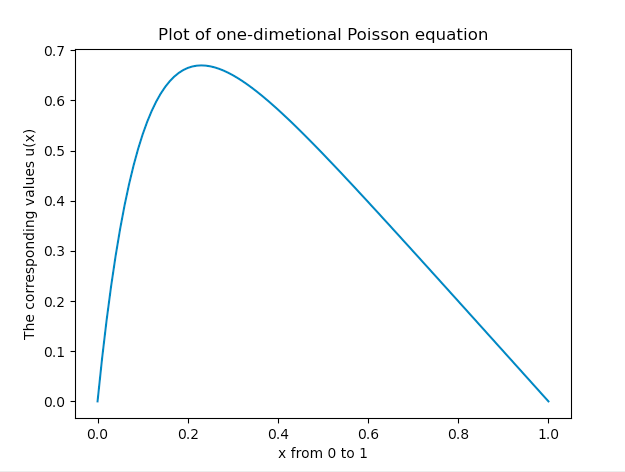
\includegraphics[scale=0.55]{Poisson} %Imports the figure.
    \caption{Plot of the one-dimentional Poisson equation with what we found to be the solution to our function $f(x)$, $u(x)$ plotted against the values of $x \in [0, 1]$. }
    \label{fig:rel_err}
\end{figure}




 \section*{Problem 3}\
 \\
In this problem we would like to discretize the Poisson equation. We start this by declaring the notation for this operation. Where we let $x \rightarrow x_i$, $u(x) \rightarrow u(x_i) \equiv u_i$, and in the end we use the term $u(x \pm h) \rightarrow u(x_i \pm h) \equiv u_{i \pm h} $. We will also use the step size h, where this is defined as the distance between two steps.
  \begin{equation}
h = \frac{1}{n - 1}.
 \end{equation}
 Where n is the number of steps we do, and therefore $x_n$ is our maximum value. We can also then use this to define each step.
  \begin{equation}
x_i = x_0 + ih, \ \ \ \ \ \ (i = 0,1, ..., n).
 \end{equation}
 Now we will look at the Taylor approximation to find our second derivative, we use the Taylor approximation with the cases $u(x + h)$ and $u(x - h)$.
 \begin{align*}
u(x + h) &= u(x) + u'(x)h + \frac{1}{2} u''(x)h^2 + \frac{1}{6} u'''(x)h^3 + O(h^4) \\
u(x - h) &= u(x) - u'(x)h + \frac{1}{2} u''(x)h^2 - \frac{1}{6} u'''(x)h^3 + O(h^4)
 \end{align*}
 Now we add the two terms $u(x + h) + u(x - h)$, so that we are left with one expression, that we rearrange, so that we get,
 \begin{align*}
u(x + h) + u(x - h) &= 2u(x) + u''(x)h^2 + O(h^4) \\
u''(x) &= \frac{u(x + h) + u(x - h) + 2 u(x)}{h^2} + O(h^2)
 \end{align*}
Now we discretize this expression using the notation we presented earlier. We know h is one step, so $\pm h$ can be represented as $\pm 1$ step. Then we find that the second derivative to be,
\begin{equation}
u''_i = \frac{u_{i +1} - 2u_i + u_{i - 1}}{h^2} + O(h^2).
\end{equation}
Which for the poisson equation then will be,
\begin{equation}
-\frac{u_{i +1} - 2u_i + u_{i - 1}}{h^2} + O(h^2) = f_i.
\end{equation}
We can do an approximation, leaving out the rest of the Taylor terms left in the $O(h^2)$ term, and change the notation from u to v, and multiply by h, so that we get a clean expression for the one-dimentional poisson equation.
\begin{equation}
-v_{i +1} + 2v_i - v_{i - 1} = h^2 f_i.
\end{equation}
We can insert our function $f(x)$ to get the special occation we are looking at,
\begin{equation}
-v_{i +1} + 2v_i - v_{i - 1} = h^2 \cdot 100 e^{-10x_i}.
\end{equation}

 \section*{Problem 4}\
 \\
Now we can use the discretized formula (8) we ended up with in problem 3 to create a matrix $\mathbf{A}\vec{v} = \vec{g}$. We use our 5 points that we used for the table in problem 2, letting i go from 0 to 5, $x_0$ to $x_5$. We already know the endpoints, $u(0) = 0$ and $u(1) = 0$, so our remaining unknown steps is the four middle points. We write these lines down and rearrange them slightly so that we get the equations,
 \begin{align*}
( i = 1): 2v_1 - v_2 &= h^2 f_1 + v_0\\
( i = 2): -v_1 + 2v_2 - v_3 &= h^2 f_2 \\
( i = 3): -v_2 + 2v_3 - v_4 &= h^2 f_3\\
( i = 4): -v_3 + 2v_4 &= h^2 f_4 v_5
 \end{align*}
Now if we let v be a vector containing the values $\vec{v} = (v_1, v_2, v_3, v_4)$. We can multiply this with the numbers we have in the equations in a matrix equation. We rearrange the right hand side of the equation as well by adding the various f values to a new vector we call g, $\vec{g} = (h^2 f_1 + v_0, h^2 f_2, h^2 f_3, h^2 f_4 v_5) = (g_1, g_2, g_3, g_4)$. Now we rearrange it all onto the form $\mathbf{A}\vec{v} = \vec{g}$.
\begin{equation}
\begin{bmatrix}
2 & -1 & 0 & 0 \\
-1 & 2 & -1 & 0 \\
0 & -1 & 2 & -1 \\
0 & 0 & -1 & 2
\end{bmatrix}
\cdot
\begin{bmatrix}
v_1 \\
v_2 \\
v_3 \\
v_4
\end{bmatrix}
=
\begin{bmatrix}
g_1 \\
g_2 \\
g_3 \\
g_4
\end{bmatrix}
\end{equation}


 \section*{Problem 5}
 \subsection*{Problem a}\
 \\
In this problem we look at a vector $\vec{v^*}$ of length m that represent the complete solution of the discretized Poisson equation, with corresponding x values given by $\vec{x}$ that goes from 0 to 1 with m steps.
\begin{align*}
\vec{v} = \begin{bmatrix}
v_1 \\
v_2 \\
... \\
v_m
\end{bmatrix}
\end{align*}
In the exact solution we will therefore have a result for all the values of $\vec{v^*(x_0)}$, $\vec{v^*(x_1)}$, all the way up to $\vec{v^*(x_m)}$.
Above we did look at the possibility to compute the exact result $\vec{v}$ from the matrix A. We can then let this matrix A be an nxn matrix. Because we do not have to look at the endpoints. This is because we already know these endpoints to be $\vec{v}(0) = 0$ and $\vec{v}(1) = 0$. So that the relation between the length n and m will be, \textbf{n = m-2}.



 \subsection*{Problem b}\
 \\
 When we compute the equation $\mathbf{A} \vec{v} = \vec{g}$ We find the approximate solution to the nxn matrix A. In this solution we will only enter the second order of the equation and leave out the extra terms that makes this an approximation. Also this matrix is the nxn matrix so the solution to v will be without the endpoints.




 \section*{Problem 6}
 \subsection*{Problem a}\
 \\
 For problem 6 we will look at the system where we find $\vec{v}$ from the multiplication of the matrix \textbf{A} and the known vector $\vec{g}$, $\mathbf{A}\vec{v} = \vec{g}$. We start with the matrix from equation(10). Where we change the notation for for the diagonal to the variable b, then the upper diagonal to a and the lower to c, so that these variables has the values, $b = 2$, $a = -1$ and $c = -1$. We write up this matrix A, and the rest of the equation.
\begin{align*}
 \begin{bmatrix}
 b_1 & c_1 & 0 & 0 \\
 a_1 & b_2 & c_2 & 0 \\
 0 & a_2 & b_3 & c_3 \\
 0 & 0 & a_3 & b_4
 \end{bmatrix} \begin{bmatrix}
 v_1\\
 v_2\\
 v_3\\
 v_4
 \end{bmatrix} = \begin{bmatrix}
 g_1\\
 g_2\\
 g_3\\
 g_4
 \end{bmatrix}
\end{align*}
 To solve this equation we will be using forward substitution to make an equation so that all the a's will be replaced by zeros. We being with $a_1$ and change up the values around by doing multiplying the row with itself $\pm$ some constant times the row above. and then we repeat this for all the rows. We see that the changes we do will be,
 \begin{align*}
 R_2 &\rightarrow R_2 - \bigg(\frac{a_2}{\tilde{b}_1} \bigg) R_1\\
 R_3 &\rightarrow R_3 - \bigg(\frac{a_3}{\tilde{b}_2} \bigg) R_2\\
 R_4 &\rightarrow R_4 - \bigg(\frac{a_4}{\tilde{b}_3} \bigg) R_3\\
 \end{align*}
 From this we see that we have a pattern, and we can rewrite this into an algorithm that we can use later, see equation(11).
 \begin{equation}
 R_i \rightarrow R_i - \bigg(\frac{a_i}{\tilde{b}_{i - 1}} \bigg) R_{i - 1}
 \end{equation}
 In this equation we have some variables we have not yet declared. These comes from the equations we do and we have that,
 \begin{align}
 \tilde{b_1} &= b_1\\
 \tilde{b_2} &= b_2 - \frac{a_2}{\tilde{b_1}}c_1\\
 \tilde{b_3} &= b_3 - \frac{a_3}{\tilde{b_2}}c_2\\
 \tilde{b_4} &= b_4 - \frac{a_4}{\tilde{b_3}}c_3.\\
 \end{align}
 From this we find a general formula,
\begin{equation}
  \tilde{b_i} = b_i - \frac{a_i}{\tilde{b_{i-1}}}c_{i - 1},
\end{equation}
 where $ \tilde{b_1} = b_1$ is the initial value.
 Now we would have to update our g values aswell,
 \begin{equation}
 \tilde{g_i} = g_i - \frac{a_i}{\tilde{b_{i-1}}}\tilde{g_{i-1}}
 \end{equation}
where the initial value is $\tilde{g_1} = g_1$.
Now we keep going with backward substitution, where we start with the last row and do equations upwards. We are now left with a matrix with only zeros in the lower triangle of the matrix. This means that we already have the value $\tilde{b_4}$. We write up this matrix notation to keep track on where we are.
\begin{align*}
 \begin{bmatrix}
 \tilde{b_1} & c_1 & 0 & 0 \\
 0 & \tilde{b_2} & c_2 & 0 \\
 0 & 0 & \tilde{b_3} & c_3 \\
 0 & 0 & 0 & \tilde{b_4}
 \end{bmatrix} \begin{bmatrix}
 v_1\\
 v_2\\
 v_3\\
 v_4
 \end{bmatrix} = \begin{bmatrix}
 \tilde{g_1}\\
 \tilde{g_2}\\
 \tilde{g_3}\\
 \tilde{g_4}
 \end{bmatrix}
\end{align*}
From this we see that our last value of v is known.
\begin{equation}
\tilde{b_4} \cdot v_4 = \tilde{g_4} \rightarrow v_4 = \frac{\tilde{g_4}}{\tilde{b_4}}
\end{equation}
We do the backwards operations upwards the whole way until we have only the identity matrix left. The row operations we do will then be,
\begin{equation}
R_i \rightarrow \frac{R_i  - c_i R_{n - i}}{\tilde{b_i}}
\end{equation}
Somehow we need this array to be performed backwards in a loop, i tried implement this with the index n-i which would be the last, then the next last, and so on as i increases. This leads to the different v-values for our vector. And the general form of this is listed in eqution(21).
\begin{equation}
  v_i = \frac{\tilde{g_i} - c_i v_{n - i}}{\tilde{b_i}}.
\end{equation}


 \subsection*{Problem b}\
 \\
Now we want to figure out the number of floating point operations in this algorithm. We find the number of FLOPs in each process and add them together. We start by the forward substitution. In each row process we have a division, a multiplication and a subtraction. Which means there will be 3 FLOPs times the number of row operations we do.  For each row operation we also update the b value and the g value, where the update of the b value has 3 FLOPs, and g the same, which gives all these processes 3n FLOPs. Now we do the same for the backwards substitution. For each row operation we have 4 FLOPs, and for all these row operations we compute the v value, which have 4 more FLOPs, with n rows we then get that this gives 4n FLOPs for each of these processes. %If we add all these FLOPs together we have that the whole algorithm for finding v would take 15n FLOPs.














 \section*{Problem 7}
 \subsection*{Problem a}\
 \\
 We write a program based on the Thomas Algorithm we created over. I have used quantstart as template to create my code from.\textsuperscript{1} From this I have adjusted the template slightly to our project and to print to file in the format I would like. We print out N = 6 steps to table(2), to compare to the exact solution we found in problem 2.
 \begin{table}%[h!]
    \centering
    \caption{Poisson: x values with corresponding v(x) values.}
    \begin{tabular}{c@{\hspace{1cm}} c}
        \hline
        x & v(x) \\
        \hline
        0.0 &  0.00\\
        0.1 & 63.5288\\
        0.2 & 68.2262\\
        0.3 & 62.9661\\
        0.4 & 54.0429\\
        0.5 & 43.7721\\
        0.6 & 33.0056\\
        0.7 & 22.0567\\
        0.8 & 11.0407\\
        0.9 & 0.0 \\
        1.0 & 0.0 \\
        \hline
    \end{tabular}\label{tab:output_table}
\end{table}
 \subsection*{Problem b}\
 \\
Now we can adjust out N value from 10, 100 to 1000. I use 100 points to make a plot that is compareble to the one we made in problem 2. We can see the plot of this in figure(2).
\begin{figure}%[h!]
    \centering %Centers the figure
    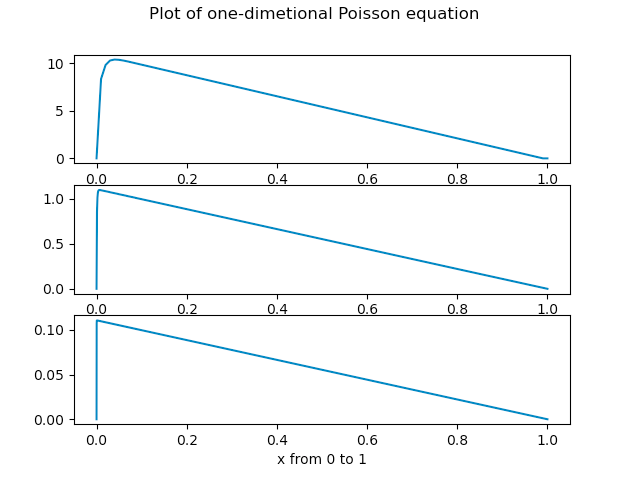
\includegraphics[scale=0.55]{v_av_matrise} %Imports the figure.
    \caption{Plot of the one-dimentional Poisson equation with what we found to be the solution to our function $f(x)$, $v(x)$ using the thomas algorithm of the $\mathbf{A}\vec{v} = \vec{g}$, plotted against the values of $x \in [0, 1]$. From above we have the first plot to be with N = 100, then N = 1000, and in the end N = 10000.}
    \label{fig:rel_err}
\end{figure}
Now when we look at the figure there is something in the code that changes slightly when the N increses. The values seems to be changing from going from 0 to 1, to with 100 go from 0 to 10. We change this in the code by dividing on 10, but this gives us something wring in the output value. Iguess anyway we see the shape of the print. But excactly what the error comes from I havent figured. i therefore will compare from the N = 100 plot, when this is the same as in problem 2.














  \section*{Problem 8}\
 \\
 In this problem I added my u values and v values and found the absolute error x and the relative error, w, from the equations,
  \begin{align*}
x &= |u_i - v_i | \\
w &= \bigg| \frac{u_i - v_i}{u_i} \bigg|
 \end{align*}

 And made a program error.cpp, where I find the values of u, v, $log_{10}(x)$ and $log_{10}(w)$, which we can see in table(3). Now we plot the absolute error together with the x-values for different choices of N. We use the template program from Anders's github page to compute the error analysis, and his plot on this. We see the plot in figure(?).





 These values if I had time I would be taking the logarithm of and made plots of, but I didn't have enough time to complete either this or the last two tasks of this problem set. I am aware that this problem set has loads of holes, and if it weren't for the fact that I have to deliver now I would definitely finished this in a better way. Hopefully there is enough within this problem set to let me pass. I haven't had much days completing this task and haven't had the time to get help from group lessons due to time, and therefore loads of my programs have bits from googling issues, which if I had time I should have written down the links from. Hopefully this will not give me any issues!
\begin{table}%[h!]
    \centering
    \caption{u-values, v-values, the relative error w and the absolute value x}
    \begin{tabular}{c@{\hspace{1cm}} c c c}
        \hline
         u & v & $log_{10}(w)$ & $log_{10}(x)$ \\
        \hline
  5.3212500000e-01  & 3.1764400000e-01 & -3.9462483734e-01 & -6.6861117416e-01\\
  6.6467400000e-01  & 6.3528800000e-01&  -1.3544682166e+00  &-1.5318595257e+00\\
  6.5022700000e-01 & 6.8226200000e-01 & -1.3074402708e+00  &-1.4943752717e+00\\
  5.8170300000e-01 & 6.2966100000e-01 & -1.0838402402e+00 & -1.3191389366e+00\\
  4.9328500000e-01 & 5.4042900000e-01&  -1.0196714814e+00  &-1.3265735719e+00\\
  3.9754800000e-01 & 4.3772100000e-01 & -9.9545530817e-01  &-1.3960657352e+00\\
  1.9970100000e-01 & 3.3005600000e-01 & -1.8525254563e-01 & -8.8487230603e-01\\
  9.9917500000e-02 & 2.2056700000e-01 & 8.1883967254e-02 & -9.1847447357e-01\\
        \hline
    \end{tabular}\label{tab:output_table}
\end{table}













\begin{thebibliography}{1}

  \bibitem{notes} Quantstart {\em https://www.quantstart.com/articles/Tridiagonal-Matrix-Algorithm-Thomas-Algorithm-in-C/}



  \end{thebibliography}


\end{document}
